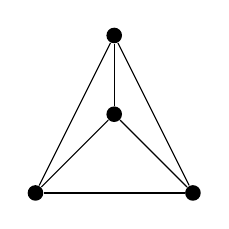
\begin{tikzpicture}
\tikzset{knoten/.style={circle,fill=black,inner sep=0.7mm}}
\node [knoten] (a) at (0,0) {};
\node [knoten] (b) at (2,0) {};
\node [knoten] (c) at (1,2) {};
\node [knoten] (d) at (1,1) {};
\draw[-] (a) to (b);
\draw[-] (c) to (a);
\draw[-] (d) to (c);
\draw[-] (a) to (d);
\draw[-] (b) to (c);
\draw[-] (b) to (d);
\end{tikzpicture}